\documentclass[conference]{IEEEtran}
\IEEEoverridecommandlockouts
\usepackage{cite}
\usepackage{amsmath,amssymb,amsfonts}
\usepackage{algorithmic}
\usepackage{booktabs}
\usepackage{wrapfig}
\usepackage{graphicx}
\usepackage{tablefootnote}
\usepackage{hyperref}
\usepackage{subcaption}
\usepackage{caption}
\usepackage{svg}
\graphicspath{ {./figures/} }
\usepackage{textcomp}
\usepackage{xcolor}
\usepackage{url}
\usepackage[autostyle]{csquotes}
\begin{document}

\title{\textit{Tweets} Sentiment Analysis}

\author{\IEEEauthorblockN{Giuseppe Concialdi}
\IEEEauthorblockA{\textit{Politecnico di Torino} \\
Student id: s294666 \\
giuseppe.concialdi@studenti.polito.it}
\and
\IEEEauthorblockN{Christian Montecchiani}
\IEEEauthorblockA{\textit{Politecnico di Torino} \\
Student id: s303681 \\
christian.montecchiani@studenti.polito.it}
}

\maketitle

\begin{abstract}
 
\end{abstract}

\section{Problem overview}\label{sec:overview}
The objective of the competition was to build a model that is able to classify whether a tweet contains positive or negative sentiments. The dataset provided is arranged as follow:
\begin{itemize}
    \item A \textbf{development} set composed by 224,994 records of tweets. Each sample has six different features, including the \textit{sentiment} attribute that is the target of the classification.
    \item A \textbf{evaluation} set consisting of 74,999 samples. It does not contain the target variable.
\end{itemize}
%\textbf{***move}The dataset is quite large, so the time required to manage the operations on the data should be taken into account because it could be not trivial. It is essential to retrieve some meaningful information of the data by exploiting its features.
Every sample is characterized by:
\begin{itemize}
    \item \textit{ids}: the unique identifier of the tweet. It is represented by a progressive integer number that is related to the timestamp of the tweet. By digging in the past twitter documentation, we found out that the tweet id is generated with a snowflake schema\cite{snowflake}, invented by Twitter for the generation of sequential ids for their tweets.
    \textbf{***add schema}
    \item \textit{date}: the timestamp of each tweet. %The date is encoded as a string with the format:
    %$$weekday \quad month \quad day \quad hour:min:sec \quad tz \quad year$$
    %From this schema, the information can be easily extracted and exploited to train the model.
    The dates in the dataset range from April 6 to June 25 of 2009. Knowing the temporal ranges will help during the preprocessing phase.
    \item \textit{flag}: a string whose significance is unsure. It is present in the whole dataset with the unique value of \texttt{NO\_QUERY}. %Given its absence of meaning, this feature will be removed without a second thought, but it is possible that it would report the query used to retrieve the tweets when they were extracted using some Twitter APIs.
    \item \textit{user}: the username of the creator of the tweet. Even though there are almost 225 thousand tweets, there are only 10,647 different usernames. %Therefore, on average, the users are very active and they have probably posted several tweets in this period.
    \item \textit{text}: the text of the tweet. This is the core part of the analysis, it embodies a lot of insights that can be extracted and analyzed to retrieve the overall polarity of the tweet's sentiments. In 2009 the maximum length of a tweet was 140 characters\cite{tweet_lenght}. However Figure \ref{fig:charcount}, shows that some tweets exceed this threshold, so there are likely issues with the encoding of the text extracted.
    \item \textit{sentiment}: the target variable of the classification. It assumes two possible integer values: 0 and 1 that represent respectively negative and positive sentiments. The dataset is fairly unbalanced, as shown in figure \ref{fig:unbalanced}, there are more positive sentiments than negative ones.
\end{itemize}
\begin{figure}[h]
        \centering
        \includesvg[width=\columnwidth]{charcount}
        \caption{Boxplot showing the number of chacters of the tweets per sentiment}
        \label{fig:charcount}
\end{figure}
\begin{figure}[h]
        \centering
        \includesvg[width=\columnwidth]{unbalanced}
        \caption{Distribution of the tweets' sentiments in the training dataset}
        \label{fig:unbalanced}
\end{figure}
The dataset does not feature any missing value, but it contains redundant information that is useless for the analysis.

In Section \ref{sec:approach} we will assess what are the most relevant features to carry on the classification and how we will extract the relevant information that lies within each feature.

\section{Proposed approach}\label{sec:approach}
The preprocessing was characterized by the features extraction and the text mining phases.

We decided to extract the time-related information from the \textit{date} attribute. 
At this stage was still unknown whether all these attributes extracted from the \textit{date} variable would have been useful or not. That is because the \textit{ids} feature is not useless, but it already encodes the timestamp of the tweet. Nonetheless, we decided to leave those features and figure out later if their relative importance would matter.

Although the \textit{date} attribute could hide some useful insights about the sentiment of the tweet, the major knowledge lies within the \textit{text} attribute. The information extraction from this feature can be performed in different ways and with different processes. We decided to tackle the problem from different points of view and we managed to embed all this data into our model. Firstly, we cleaned up and fix some problems present in the tweets' text, then we exploited the text performing:
\begin{itemize}
    \item A \textbf{sentiment intensity analysis}\cite{sentiment_analysis} on the text, obtaining new features on the polarization of the sentiments.
    \item A \textbf{tf-df}\footnote{Term Frequency - Document Frequency. The tf-df of term $t$ in document $d$ of collection $D$ is computed as: $$tfdf(t) = freq(t,d) * \log(freq(t,D)$$} of the text in order to get the words that mainly influence the sentiments of the tweets.
    \item A \textbf{word embeddings}\cite{wordembeddings} approach with the FastText\cite{fasttext} library to retrieve the morphological relationships between the words in a sentence.
\end{itemize}
\begin{figure}[h]
        \centering
        \includesvg[width=\columnwidth]{overall_schema}
        \caption{Overall schema of the problem approach}
        \label{fig:overall_schema}
\end{figure}
Figure \ref{fig:overall_schema} shows a summary of our approach.
The last technique resulted in a very powerful tool, that is able, on its own, to perform the classification of the sentiment of the evaluation set with a macro F1-score\footnote{The F1-score is the harmonic mean of the precision and recall therefore it is defined for a single class. With macro F1-score we refer to the mean of all classes' F1-scores.} higher than 0.8. This was our baseline for the development of the model, and we accomplished higher performance by integrating the likelihoods of the FastText supervised learning classification\cite{fasttextclassifier} into our dataset. 

Sections \ref{sec:preprocessing} and \ref{sec:model} will dig into the details of the three different text mining techniques and some comments about the word embedding can be found in the Discussion section \ref{sec:discussion} of the paper.

\subsection{Preprocessing}\label{sec:preprocessing}
The preprocessing step is the core phase of the entire analysis. Here we performed the extraction, transformation and normalization of the features. As discussed in Section \ref{sec:approach}, we extracted from the \textit{date} attribute all the relevant information and we discarded the properties that are redundant like \textit{year}, \textit{timezone} and \textit{flag}. Then we decided to add a new feature based of the number of characters of the tweet. The new \textit{char\_count} attribute is useful to troubleshoot the tweets' texts that are longer than 140 characters and it is also valuable for the classification itself.

Afterwards, we addressed the tweet duplication issue. There are three kinds of duplicated tweets:
\begin{enumerate}
    \item Same text, different id, same sentiment
    \item Same text, same id, same sentiment
    \item Same text, different sentiment
\end{enumerate}
For the first kind of duplicated tweets, no action is required. Those are very common and eventually short sentences that different authors twitted. They share the same sentiment so it enforces the model to learn that those phases belong to one specific class. The second kind are tweets that have been posted more than once by the same author. This could be a mistake or maybe the user wanted to retweet the same post again. Either way, we decided to keep only one copy of the duplicated post. The most controversial kind of duplication is the last one: regardaless of the author, if the same text is labelled differently, then the classifier will be confused on how to handle samples similar to these ones. For this reason we decided to drop all the records with these conflicting properties.

Then, we tackled the cleaning of the tweets' text. To properly perform this step, we took into consideration a lot of alternatives. Different elements characterize a Twitter post and we tried to draw every possible bit of information from the text. The tweets' length issue led us to inspect the text in search of an encoding-related problem. We found out that the text extracted seems to be encoded in UTF-8\cite{utf8} but some special symbols were parsed as HTML entities\footnote{Character entities are used to display reserved characters in HTML}. We employed the html library to clean up the text. After that, we lowered the case of the words and we extracted the domain name from the urls contained in the tweets. We exploited two vocabularies\footnote{\textbf{***insert libraries}} to expand into clear words the emoticons and the slang terms. By substituting these pieces of text in addition with some regex to regularize the phrases we obteined a much more coherent and convenient format for the analysis. Ultimately, we applied the lemmatization\cite{lemmatization} to extract the lemma from each word. We preferred lemmatizing to stemming\cite{stemming} in order to preserve the morphology of the words\cite{stemmingVSlemmatizing}.
Figure \ref{fig:cleaning} shows the cleaning pipeline for the \textit{text} attribute.

At this stage, the \textit{text} feature is ready to be processed. We heavily relied on the tools offered by the NLKT library\cite{nlkt} to carry on the analysis. We employed the Vader Sentiment Intensity Analyzer\cite{vader} to gain the relative frequencies of \textit{negative}, \textit{neutral} and \textit{negative} terms. Besides, also the \textit{compound} value is stored, it is a single value summarises the three frequencies. Following, we used the TextBlob library\cite{textblob} to extract additional features: the \textit{subjectivity} score and the \textit{polarity} index. These variables are correlated among them, but they describe the same phenomenon under different point of view and complement each other.

Going forward, we applied a TF-DF to the text word with a relative high minimum support. Our aim was to retrieve the words that were present in a lot of tweets and which meaning was heavily polarized toward one class. In this case, we did not use a normal stop words vocabulary, because there are a lot of common term that are very important for the classification, like the negations. So we created a custom vocabulary that contained only conjunctions and some adverbs. The results of the TF-DF are shown in Figure \ref{fig:word_cloud}
\begin{figure}[h]
        \centering
        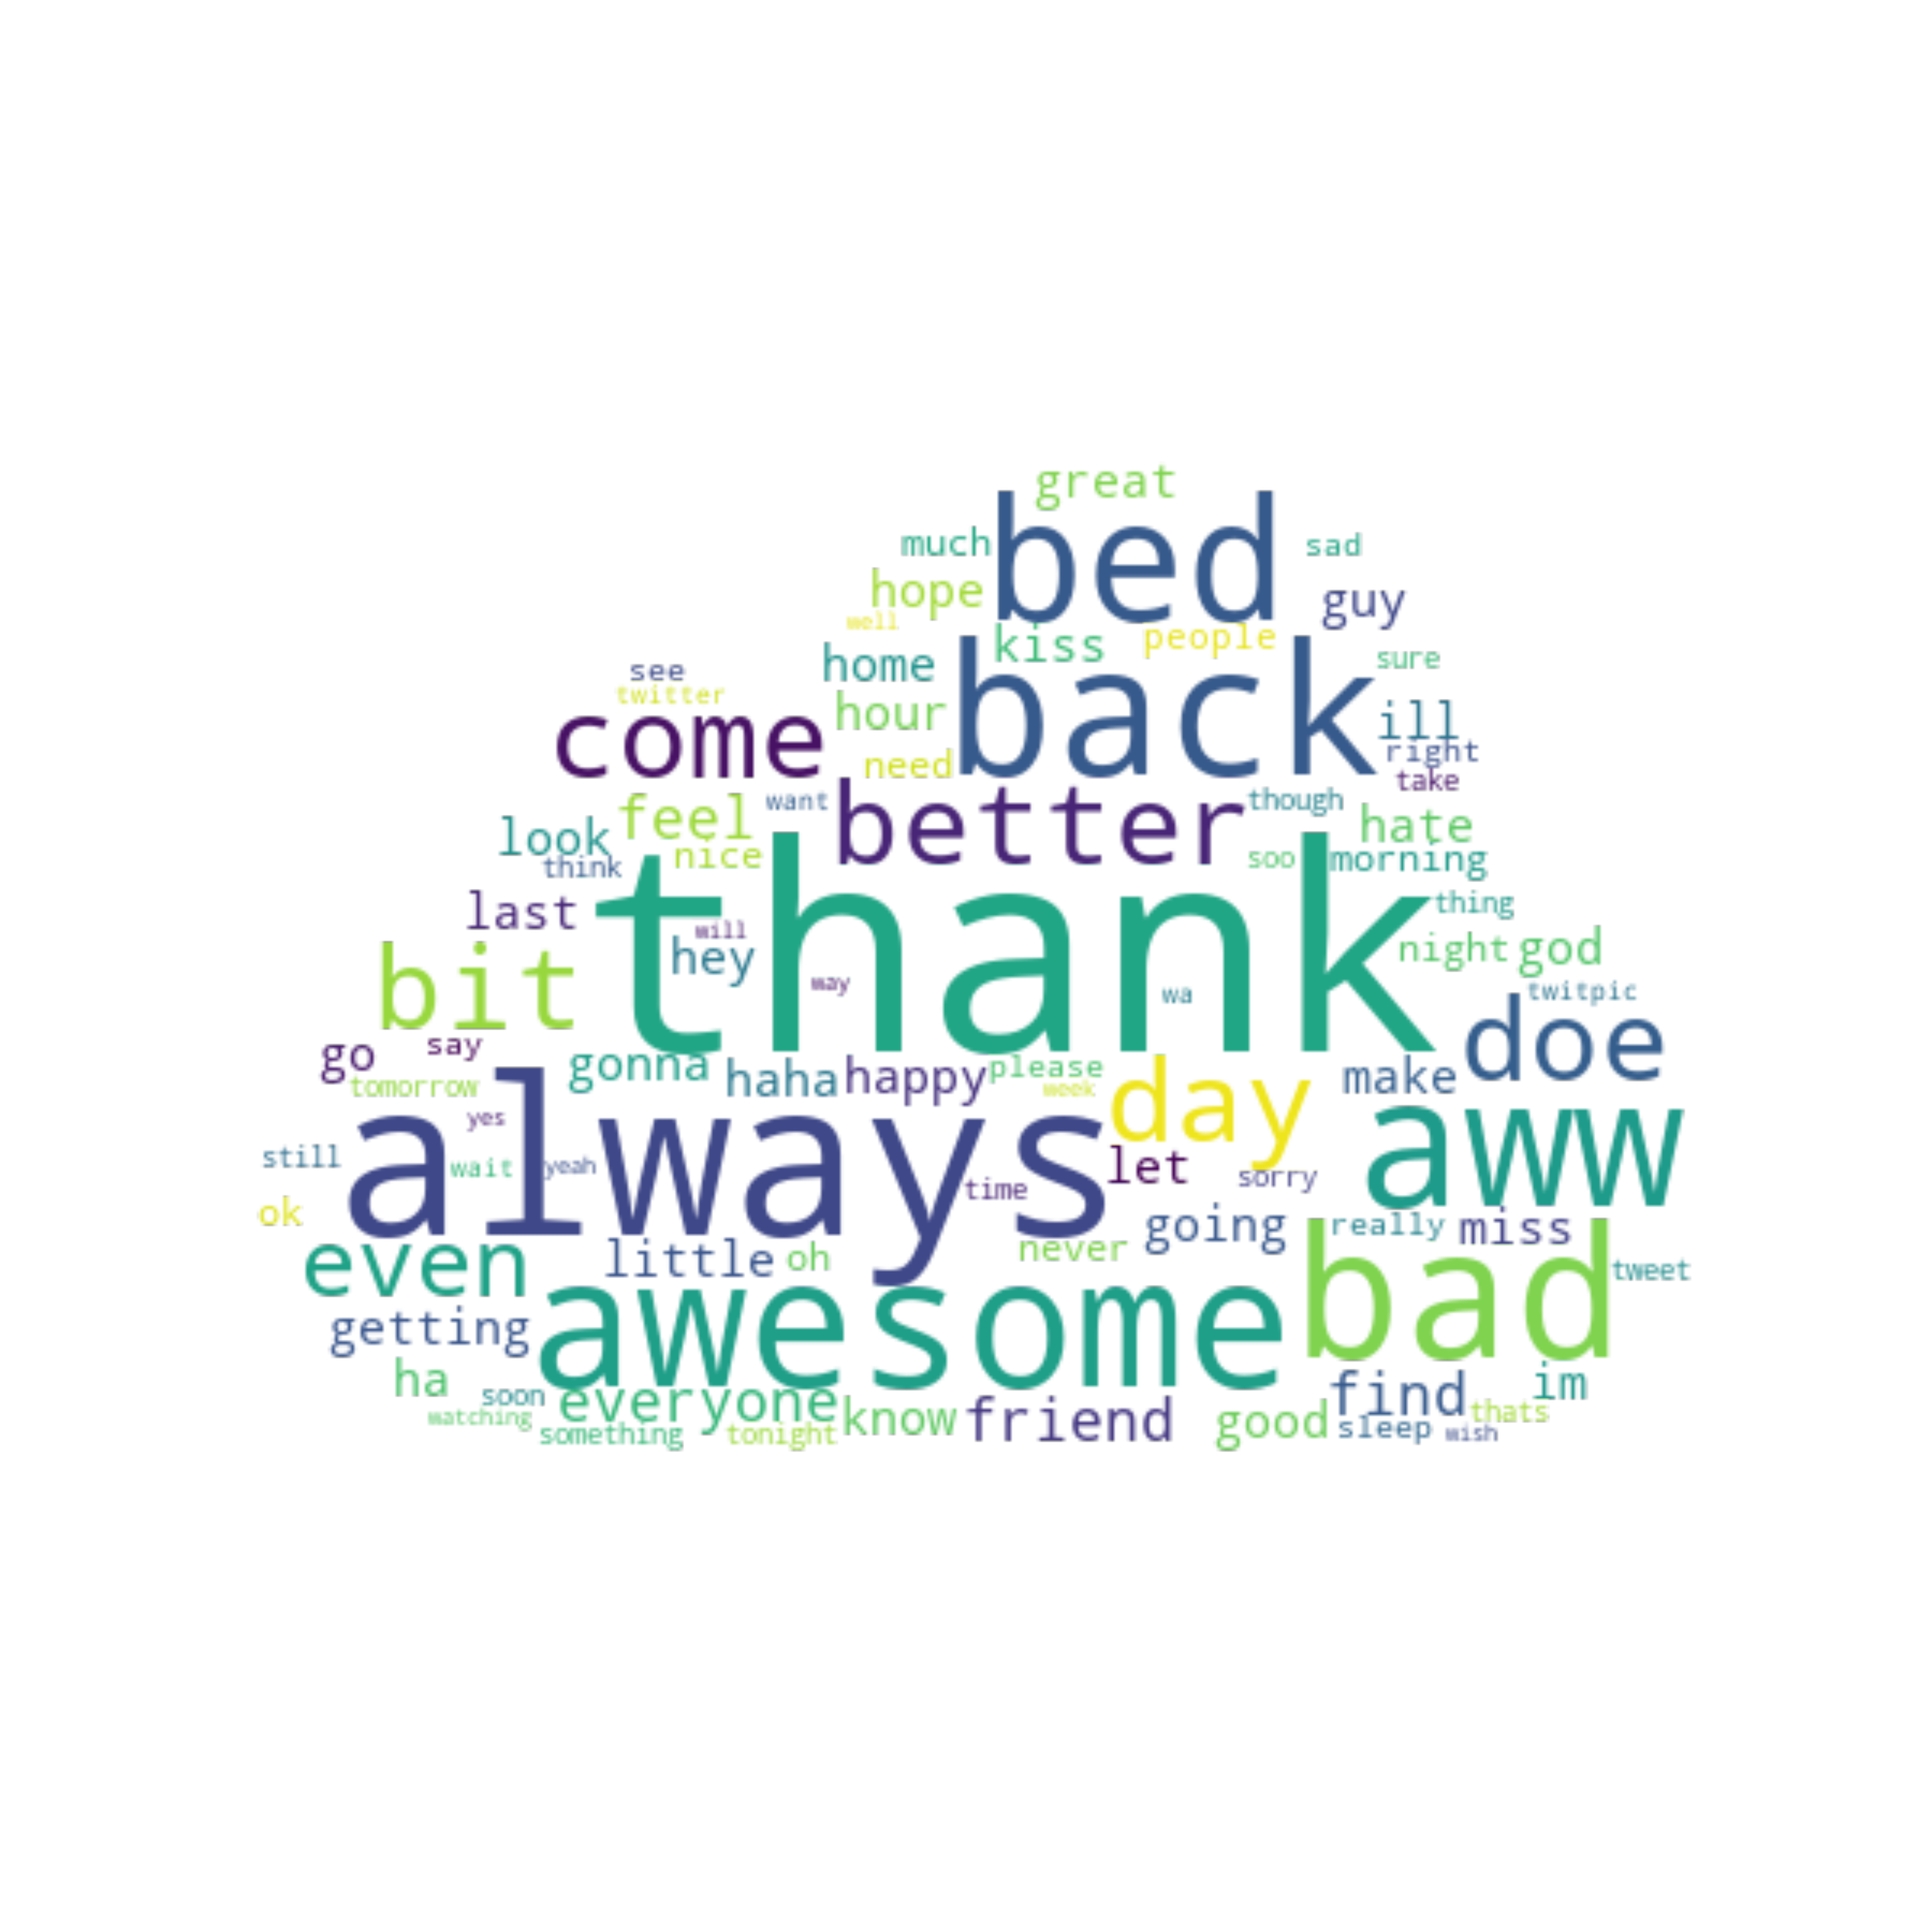
\includegraphics[width=\columnwidth]{word_cloud}
        \caption{Word Cloud generated by the results of the TF-DF. The figure has been created using the wordcloud library\cite{word_cloud}}
        \label{fig:word_cloud}
\end{figure}
Finally, we leveraged the word embeddings approach through Meta's FastText library. The vocabulary was built on top of the tweets of the development set. The autotuning feature of the library allowed us to treat the neural network underneath the facade as a black box. We split the development data into training and validation and the model tuned itself by maximizing the resulting f1-score. One of the strenghts of this technique is that by converting the words into multi-dimensional vectors it does not suffer the presence of unfamiliar terms. The output of the neural network is a prediction and the softmax likelihood for each class. We extracted these probabilities and we integrated them into the dataset.
\begin{figure}[h]
        \centering
        \includesvg[width=\columnwidth]{text_schema}
        \caption{Feature extraction schema of \textit{text} attribute}
        \label{fig:text_schema}
\end{figure}
Figure \ref{fig:text_schema} summarises the operations perfomed on the \textit{text} attribute.

The data is not yet ready to be processed by a classification algorithm. The categorical needs to be addressed. We removed the \textit{text} and the \textit{user} features because we have already extracted the information needed and then we proceed to map the remaining features into numerical ones. All the columns are normalized with a MinMax scaler\cite{minmax} and it is ready to go through the model selection pipeline.
\subsection{Model selection}\label{sec:model}
We chose four different algorithms to perform the classification task and we compared their performances to assess which are the best classificators to perform this job:
\begin{itemize}
    \item \textbf{Random Forest Classifier\cite{rf}}: ensemble of decision trees.
    \item \textbf{Bernoulli Naïve Bayes\cite{bnb}}: classifier for multivariate Bernoulli\cite{bernoulli} models.
    \item \textbf{Linear Support Vector Classifier\cite{svc}}: linear kernel version of the more general SVC.
    \item \textbf{Histogram-based Gradient Boosting Classification Tree\cite{histgtb}}: high-performance implementation for big datasets of the Gradient Tree Boosting Classifier\cite{gtb}. 
\end{itemize}
To test the effectiveness of our preprocessing, we tried to test the performances of the models by increasingly combining the results of the different techniques applied to the \textit{text} attribute. As it is possible to see in Table \ref{tab:results}, at first we applied only the word embeddings approach, then we joined it with the sentiment extraction results and in the last trial, we added the TF-DF outcomes into the equation. It is possible to see that our baseline with the word embeddings provides a fairly high F1-score. The highest score is reached by bringing together all the extracted features with the different methods.

During this phase, we exploited the Random Forest feature importances to understand what are the most relevant features upon which the algorithm is splitting the samples. Accordingly to our results, we found out that the most significant attributes are the likelihood resulting by the word embeddings classification, following there are the sentiment features and lastly some very polarized word coming from the TF-DF. We also discovered that the \textit{ids} attribute was always more relevant than the feature extracted on the date, thus we decided to remove those features and leave only the id.
\subsection{Hyperparameters tuning}\label{sec:hypertuning}
- For tuning our models we first need to split the development dataset. We decide to keep 80\% of the records in the training set, and use the remaining 20\% for the test set. To optimize our models ..
The main drawback of Hist Gradient Boosting Models is the very large number of hyperparameters to be tuned. Approaching this problem with a standard grid search is computationally prohibitive. HalvingGridSearch is an hyperparameter optimization technique that tries all the candidates with a small amount of resources and iteratively selects the best candidates, using more and more resources.


\begin{table}[]
\begin{tabular}{@{}ll@{}}
\toprule
\textbf{Parameters}                    & \textbf{  Values} \\ \midrule
\multicolumn{1}{l|}{criterion}         & gini, entropy   \\
\multicolumn{1}{l|}{min\_sample\_leaf} & 20,35,60        \\
\multicolumn{1}{l|}{max\_features}     & sqrt, log2      \\ \bottomrule
\end{tabular}
\end{table}

\section{Results}\label{sec:results}
- We will now compare the results obtained with the two models, using the hyperparameters discussed in the previous section.
\section{Discussion}\label{sec:discussion}
This classification task extensively relied upon Natural Language Processing library. Every library offers a wide range of tools that allows to effectively retrieve information from the text. We decided to cover more NLP libraries to benefit from the variety of materials at our disposal. Almost every library provides advanced features, such as Part Of Speech Tagging, that could have been beneficial to the classification but we decided not to include in this analysis. 

We tried to operate with the \textit{user} attribute to retrieve some useful information within it. We thought that due to the relative low cardinality of this attribute (only 10,000 different usernames) the tweets posted by the same author may reflect its personality, thus it is likely that a sentiment is predominant to the other one. Nonetheless, the One-Hot-Encoding\cite{ohe} of this features would have resulted into a huge dimensionaly increase of the dataset.

All the classification algorithm, and the majority of utilities employed in Section \ref{sec:model} and \ref{sec:hypertuning} come from the scikit-learn packages\cite{scikit-learn}. Alongside the classical classification algorithms, we decided to try the Histogram-based Gradient Tree Boosting Classifier because, like the Random Forest Classifier, it is an ensemble of decision tree. Given that the Random Forest Classifier was always among the best-performing algorithms for this task, we wanted to explore how the boosting technique would have performed for this job.
\bibliography{bibliography}
\bibliographystyle{ieeetr}

\end{document}